\chapter{自動原子削除の実装}\label{ux81eaux52d5ux539fux5b50ux524aux9664ux306eux5b9fux88c5}

粒界生成において,回転,並びに鏡映操作を行った後の原子配置を図に示した.

\begin{center}
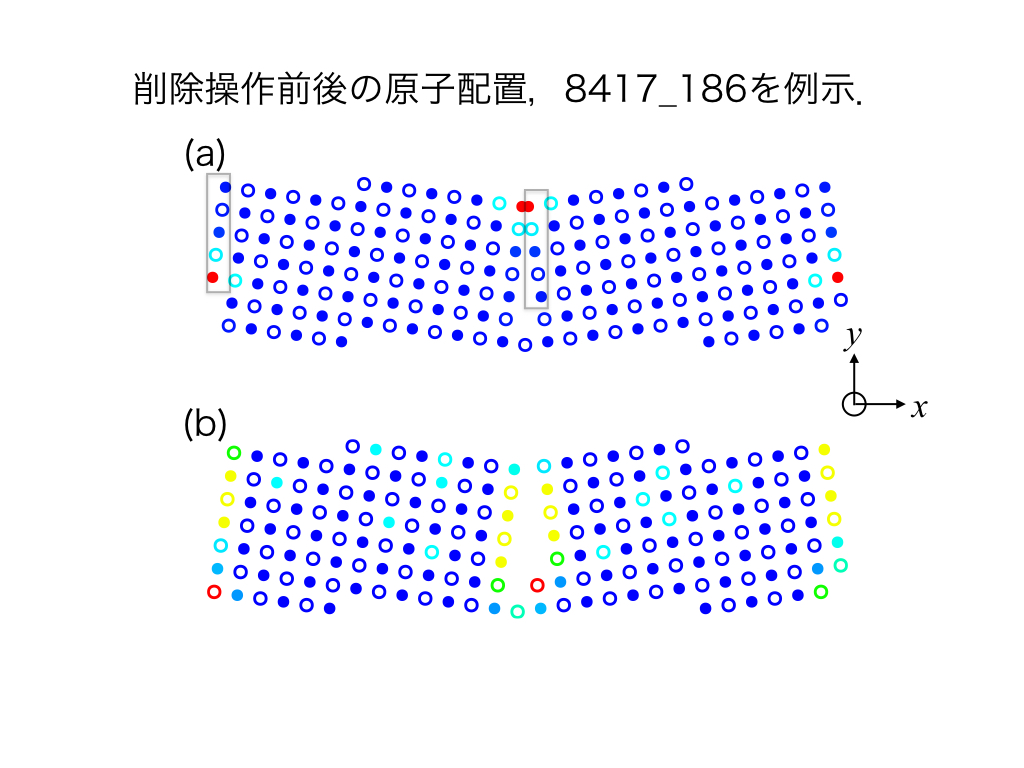
\includegraphics[width=150mm]{../.././auto_delete/auto_delete_002.jpeg}
\end{center}
削除操作前後の原子配置,8417\_186を例示.

\label{fig:}

ここでは,8417\_186を例にしている.8417の数字は粒界系全体の構造を表している.それぞれ,x=8,
y=4, z=1およびtan
\(\theta=1/7\)を意味しており,x軸方向に8x2層,y軸方向に4x2層の層を保持している.

削除操作は,このx=0, およびx=0.5つまり,系の端と真ん中あたりにある
粒界近傍において,原子が詰まりすぎているのを解消するために行う操作である.
枠線で囲った領域の原子を削除する.
これまではVestaという表示ソフトを使って,原子サイトナンバーを手動で確認し,
モデル作成司令ファイル(modeler\_8417など)に記述する必要があった.
これを自動化しようというのがここで目指す開発コードである.

    \section{energyおよびnlによる抽出}\label{energyux304aux3088ux3073nlux306bux3088ux308bux62bdux51fa}

    当初,eamのプログラムコードを流用して原子のエネルギー(:ene, energyの略)
あるいは配位数(:nl,neighbour listを意味)を使った選別を試みた.
近傍の原子を取り出すと,

\begin{verbatim}
   4   28.86278    8.28733    2.02070  11   -2.65182  0.738    3.08007   -5.73189 0.54
   5   28.57701   10.28772    0.00000  13    0.23319  3.623    7.50972   -7.27653 1.03
   6   28.29124   12.28812    2.02070  14   12.27927 15.669   21.86782   -9.58855 2.28
   8   55.72518    6.00117    2.02070  14   12.27927 15.669   21.86782   -9.58855 2.28
  94   55.43941    8.00156    0.00000  13    0.23319  3.623    7.50972   -7.27653 1.03
  95   55.15364   10.00195    2.02070  11   -2.65182  0.738    3.08007   -5.73189 0.54
 103   27.14816    8.28733    2.02070  11   -2.65182  0.738    3.08007   -5.73189 0.54
 104   27.43393   10.28772    0.00000  13    0.23319  3.623    7.50972   -7.27653 1.03
 105   27.71970   12.28812    2.02070  14   12.27927 15.669   21.86782   -9.58855 2.28
 106    0.28577    6.00117    2.02070  14   12.27927 15.669   21.86782   -9.58855 2.28
 192    0.57154    8.00156    0.00000  13    0.23319  3.623    7.50972   -7.27653 1.03
 193    0.85731   10.00195    2.02070  11   -2.65182  0.738    3.08007   -5.73189 0.54
\end{verbatim}

が選択される.これは,6列目に記されたeneryを基準に選別したものである.
しかし,サイト番号7に対応する

\begin{verbatim}
   7   56.01095    4.00078    0.00000  12   -3.39000 -0.000    1.79000   -5.18000 0.35
\end{verbatim}

がこれらの選別基準では最安定原子と同じ環境であるため,選択から外れてしまう.

    \section{x位置による選別}\label{xux4f4dux7f6eux306bux3088ux308bux9078ux5225}

そこで,x座標による選別を実装した.
初期のcodeがわかりやすいので,そのまま記すと次のようになる.

\begin{verbatim}
a_length =   56.0109463716
dx = a_length/(32+2)
a_half = a_length/2.0
if x_pos < dx or  (x_pos > a_half and x_pos < a_half + dx)
    printf("%10.5f: ", x_pos/a_length)
\end{verbatim}

削除領域の幅(dx)は層数から計算する.
中心の長さはx軸の長さ(a\_length)から計算している. これらの領域
\textgreater{} 0 \textless{} x\_pos \textless{} dx

\begin{quote}
a\_half \textless{} x\_pos \textless{} a\_half + dx
\end{quote}
を選別するのがif文以下のところである.

こうして得られた削除原子のx\_posを取り出すと,

\begin{verbatim}
> ruby auto_delete.rb converted_poscar.txt 
divide num:   32
a length  :   56.0109463716
normal dx :    0.03125
       dx :    1.75034
   2:    0.53061   29.72009
   3:    0.52551   29.43432
   4:    0.52041   29.14855
   5:    0.51531   28.86278
   6:    0.51020   28.57701
   7:    0.50510   28.29124
 107:    0.00510    0.28577
 192:    0.03061    1.71462
 193:    0.01020    0.57154
 194:    0.01531    0.85731
 195:    0.02041    1.14308
 196:    0.02551    1.42885
\end{verbatim}

となる.ここでは,2番,192番は消したくない原子である.
これは,モデルのサイズによって変わる. この調整をdivide
numによって自動計算からするか,
あるいは10原子削除というように外部入力として入れるかを検討する必要がある.

    \section{POSCARファイルの仕様}\label{poscarux30d5ux30a1ux30a4ux30ebux306eux4ed5ux69d8}

粒界の原子座標の入出力は第一原理計算ソフトVASPのPOSCARファイルを通じて行う.
そこで,POSCARファイルを直接あつかうPOSCAR classを設計する.

今後code内での変数名を用語を一致させるため,VASP標準の単語を使用する.
POSCARの仕様は \textgreater{}
http://cms.mpi.univie.ac.at/vasp/guide/node59.html

あるいはVASP manual, pp.43-4に解説されている.

\begin{verbatim}
Cubic BN         # comment line ('name' of the system)
   3.57          # universal scaling factor ('lattice constant')
 0.0 0.5 0.5     # lattice vectors
 0.5 0.0 0.5  
 0.5 0.5 0.0
   1 1           # number of atoms per atomic species (one number for each atomic species)
Selective dynamics  # 7th
Cartesian           # 7th or 8th
 0.00 0.00 0.00 T T F
 0.25 0.25 0.25 F F F
Cartesian
 0.01 0.01 0.01
 0.00 0.00 0.00
optionally predictor-corrector coordinates 
   given on file CONTCAR of MD-run
  ....
  ....
or
Cubic BN
   3.57
 0.0 0.5 0.5
 0.5 0.0 0.5
 0.5 0.5 0.0
   1 1
Direct
 0.00 0.00 0.00 
 0.25 0.25 0.25
\end{verbatim}

1から6行目に書かれた内容は上記の例にコメントで記した.

7行目は省かれる場合がある.これがあると原子ごとに設定ができる.

The seventh line switches to 'Selective dynamics' (only the first
character is relevant and must be 'S' or 's'). This mode allows to
provide extra flags for each atom signaling whether the respective
coordinate(s) of this atom will be allowed to change during the ionic
relaxation. This setting is useful if only certain 'shells' around a
defect or 'layers' near a surface should relax. Mind: The 'Selective
dynamics' input tag is optional: The seventh line supplies the switch
between cartesian and direct lattice if the 'Selective dynamics' tag is
omitted.

と説明されている.

さらに,7 or
8行目では,これ以降の原子座標の記述法としてCartesianあるいはDirectを指定する.
次の行から原子数分の座標が記される.

Directの場合は,原子位置\(\overrightarrow{R}\)は, \[
\overrightarrow{R} = x_1 \overrightarrow{a}_1 +
x_2 \overrightarrow{a}_2 +
x_3 \overrightarrow{a}_3
\]
で指定される.ここで,\(\overrightarrow{a}_{1 \dots 3}\)は三つの基底ベクトルを指す.そして,
\(x_{1 \dots 3}\)が原子座標に記された,小数点数での値である.

Cartesianの場合は, \[
\overrightarrow{R} = s \,
\left(\begin{array}{cc}
x_1\\
x_2\\
x_3
\end{array}\right)
\] で,\(s\)は2行目にかかれているuniversal scaling factorである.
その他の箇所の説明は今回使用しないので,省略する.

これらの記述に基づいて,それぞれの変数名を

\begin{verbatim}
Cubic BN         # comment
   3.57          # scaling_factor
 0.0 0.5 0.5     # lat_vec[0][0..2]
 0.5 0.0 0.5     # lat_vec[1][0..2]
 0.5 0.5 0.0     # lat_vec[2][0..2]
   1 1           # n_atoms[0..1]
Selective dynamics  # dynamics_selector
Cartesian           # direct_cartesian_switch
 0.00 0.00 0.00  # pos[0]
 0.25 0.25 0.25  # pos[1]
\end{verbatim}

とする.

    \section{auto\_delete\_poscar}\label{auto_delete_poscar}

前述のPOSCARの情報を読み込むPoscar classを使って
実装したのが次のコードである.

\begin{verbatim}
require './poscar'

file = ARGV[0] || 'POSCAR_0_8417'
poscar = Poscar.new(file)
div = ARGV[1].to_i || 32+2
printf("divide num: %4d\n", div)
printf("a length  : %15.10f\n", a_length = poscar.lat_vec[0][0])
printf("normal dx : %10.5f\n", dx = 1.0/div)

a_half = 0.5
selected = []
poscar.pos.each_with_index do |pos,i_atom|
  x_pos = pos[0]
  if x_pos < dx or  (x_pos > a_half and x_pos < a_half + dx)
    printf("%4d %10.5f\n",i_atom.to_i+1,x_pos)
    selected << i_atom
  end
end

poscar.delete_atoms(selected)
File.open('POSCAR_tmp','w') do |file|
  file.print poscar.poscar_format
end
\end{verbatim}

削除の幅は,原子層の厚さから推測できるように第2入力として指定している.
delete\_atomsはselectedで選ばれた番号の原子をPOSCARから消去する命令である.
POSCAR\_0\_4417に適用した結果は次の通りである.

\begin{verbatim}
> ruby auto_delete_poscar.rb POSCAR_0_4417 18
divide num:   18
a length  :   28.0054731858
normal dx :    0.05556
   3    0.55102
   4    0.54082
   5    0.53061
   6    0.52041
   8    0.51020
  88    0.01020
  91    0.02041
  92    0.03061
  95    0.04082
  96    0.05102
[95, 94, 91, 90, 87, 7, 5, 4, 3, 2]
10
88
\end{verbatim}

削除原子数を指定することを断念した.これには,原子のx-座標でsortして順々に選択していかねばならない.
そのsortを指定領域で実行するコードの記述が難しそうなので,今回は見送っている.


    % Add a bibliography block to the postdoc
    
    
    
    \end{document}
